
\documentclass{abgabe}
\begin{document}

\begin{questions}
    \qformat{\thequestion. \textbf{\thequestiontitle} \hfill}
    \titledquestion{Klassendiagramm Implizierungen}

    Gegeben sei folgendes UML-Klassendiagramm mit ähnlichem Kontext wie aus der ersten Aufgabe.

    Zusätzliche Annahmen:
    \begin{itemize}
        \item Jede Person hat nur einen Personalausweis.
              Wir vernachlässigen den Fakt, dass man diesen verlegen oder verlieren kann.
        \item Studierende können sich bei der Bibliothek auf Wartelisten für Bücher setzen lassen.
              Die Bibliothek benachrichtigt die Studierenden nach dem FIFO-Prinzip, wenn das Buch verfügbar ist.
              Das soll sich in der verwendeten Datenstruktur für die Assoziation zwischen Bibliothek und Studierender in der Bibliothek widerspiegeln.
    \end{itemize}

    Hinweis: Achten Sie darauf, dass die Multiplizitäten vom Code auch abgebildet werden! Zum Beispiel, dass eine Person keine Null-Referenz auf einen Personalausweis haben darf!

    \begin{center}
        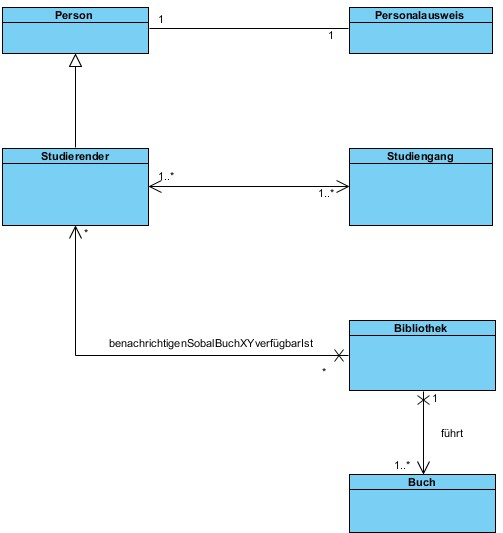
\includegraphics[width=.5\textwidth]{swt_h07_muster.jpg}
    \end{center}

    Tragen Sie in die vorgegebenen Java-Klassen, die Umsetzung der Assoziationen mit korrekter Multiplizität ein. An welchen Stellen ergibt es Sinn, die Assoziationen weiter über (unique, ordered) einzuschränken?
\end{questions}
\end{document}